
\documentclass{mcmthesis}
\mcmsetup{CTeX = true,   % 使用 CTeX 套装时,设置为 true
        tcn = 0000, problem = A,
        sheet = true, titleinsheet = true, keywordsinsheet = true,
        titlepage = true, abstract = true}
\usepackage{newtxtext}%\usepackage{palatino}
\usepackage{lipsum}
\usepackage{subfigure}
\title{The \LaTeX{} Template for MCM Version \MCMversion}
\author{\small \href{https://www.latexstudio.net/}
  {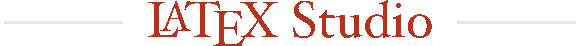
\includegraphics[width=7cm]{mcmthesis-logo}}}
\date{\today}
\begin{document}
\begin{abstract}
% 摘要


\begin{keywords}
% 关键词
keyword1; keyword2


\end{keywords}
\end{abstract}
\maketitle
%% Generate the Table of Contents, if it's needed.
%% \tableofcontents
%% \newpage
%%
%% Generate the Memorandum, if it's needed.
%% \memoto{\LaTeX{}studio}
%% \memofrom{Liam Huang}
%% \memosubject{Happy \TeX{}ing!}
%% \memodate{\today}
%% \logo{\LARGE I'm pretending to be a LOGO!}
%% \begin{memo}[Memorandum]
%%   \lipsum[1-3]
%% \end{memo}
%%

\newpage
\thispagestyle{empty}
\tableofcontents
\newpage


\section{Introduction}
\subsection{Background}
随着个人资产的累计,越来越多的人进入投资市场,为了在使现有资产保值或更有价值。
但我们都知道,投资类产品常有很强的波动性,which means它很难预测。
在众多投资产品中,黄金和比特币最受人关注。
特别是比特币,自出现以来交易规模迅速扩张,但巨大的价格波动使其安全性和稳定性受到质疑。
那么,在黄金和比特币投资热潮下,对普通交易者大幅度得利的投资组合很难实现。
这是很重要的,根据每天和前几天更新的交易数据,来预测未来波动性资产的发展趋势。
因此,交易者提出 to develop a model that uses only the past stream of daily prices 
to date to determine each day if the trader should buy, hold, or sell their assets in their portfolio.


\subsection{Problem Statement}
根据我们的理解,问题主要有以下几个要点:
\begin{enumerate}    %有序列表 
  \item 用原始数据建立一个模型,分析黄金和比特币价值走向
  \item 基于时间序列模型,预测未来波动性资产的走势
  \item 解决利用动态规划实现利益最大化问题
  \item 确定交易者每天的交易决策以及交易行为,在有交易佣金的背景下
  \item 证明我们提供了最优策略
  \item Determine how sensitive the strategy is to transaction costs
\end{enumerate}


\subsection{Problem Analysis}

明确问题后,我们的认为ARIMA模型在时间序列分析问题上较传统模型有很大优势,
工作概览如下:
首先,我们对原始数据进行了预处理,包括对数据的筛选、使数据可视化、挖掘出时间序列。
这部分的工作可以极大提高建模的效率和分析波动性资产的效率。
接着,由于在时间序列分析问题上ARIMA模型较传统模型的优势,在适用条件下我们选择ARIMA进行数据预测。
以实现资产价值最大化为目的,制定了每日买卖、调仓及投资比例。
然后,为了证明我们的策略最优,我们对制定的买卖、调仓和投资组合三个标准设置了扰动项,来确定的最佳参数。
最后,我们枚举得到的一系列结果检验了对佣金的敏感性。



\section{Assumption}





\section{Data Processing}
对于我们要解决的数据分析问题,数据的平稳性是我们的模型的基础。
通常来说,原始数据中的不完整和异常数据可能会大大影响我们问题的分析效率和结果准确性。
故,对数据的分析、预先处理是必不可少。


\subsection{Data Screening}
We analyzed the raw data in the LBMA-GOLD.csv and BCHAIN-MKPRU.csv files,final data status is as follows:


%插入图片
For the missing data in LBMA-GOLD.csv, we fill in the date according to the average of the day before and the day after.


\subsection{Data Visualization}
To observe the price trends of gold and bitcoin more visually,
we visualize the given data and draw figure\ref{fig1}and\ref{fig2}
\begin{figure}[h]
  %\small
  \centering
  \subfigure[1]{
  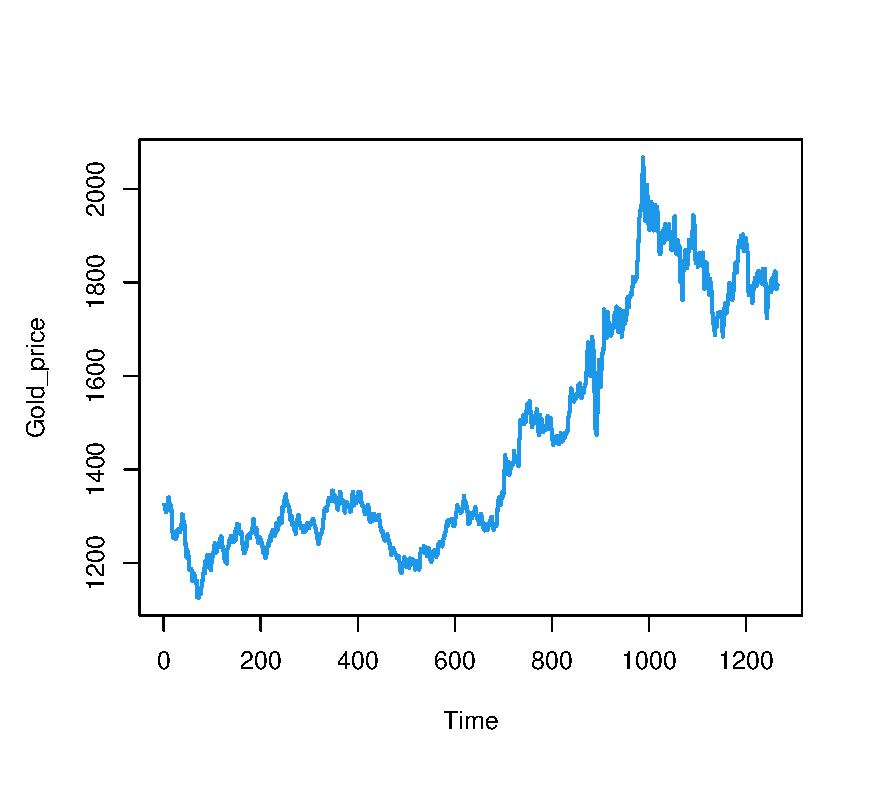
\includegraphics[width=0.9\columnwidth]{D:/meisai/ms/fig/gold.eps}}
  \caption{Gold price tendency} \label{fig1}
  %\hfill
  \centering
  \subfigure[2]{
    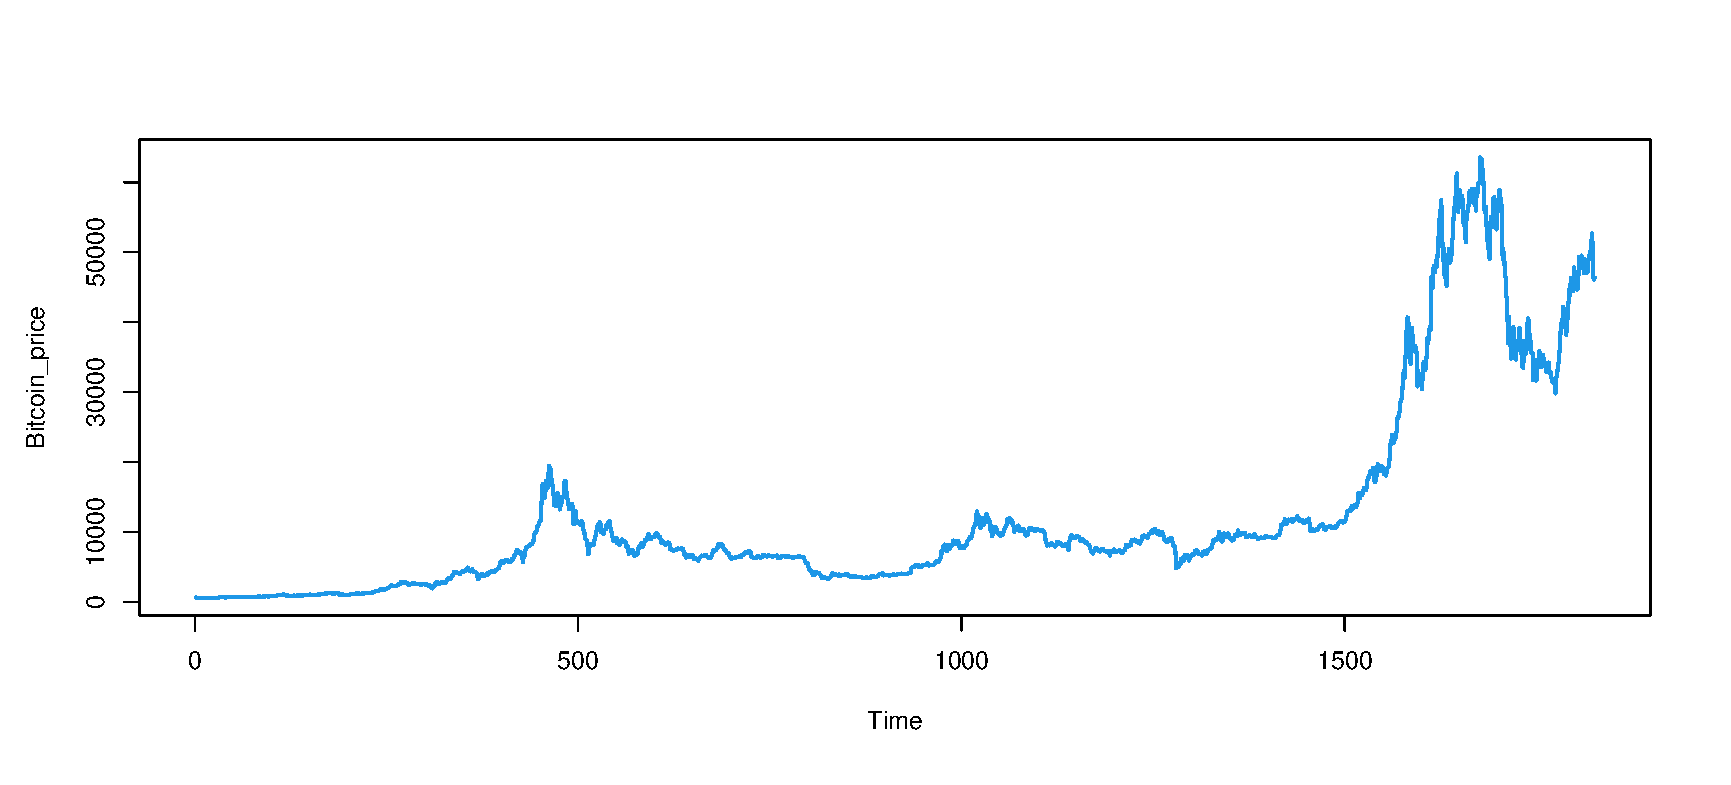
\includegraphics[width=0.9\columnwidth]{D:/meisai/ms/fig/Bitcoin.eps}}
  \caption{Bitcoin price tendency} \label{fig2}
  \end{figure}


\subsection{Mining Time Series}
For subsequent data prediction using the time series model ARIMA,
We perform stability test and white noise test on the raw data and processed data as a way to mine meaningful time series.


\subsubsection{Stability Test}
First,we test the stability of the original data by comparing two methods, the image observation and the unit root test.

\begin{figure}[!hb]
  \centering 
  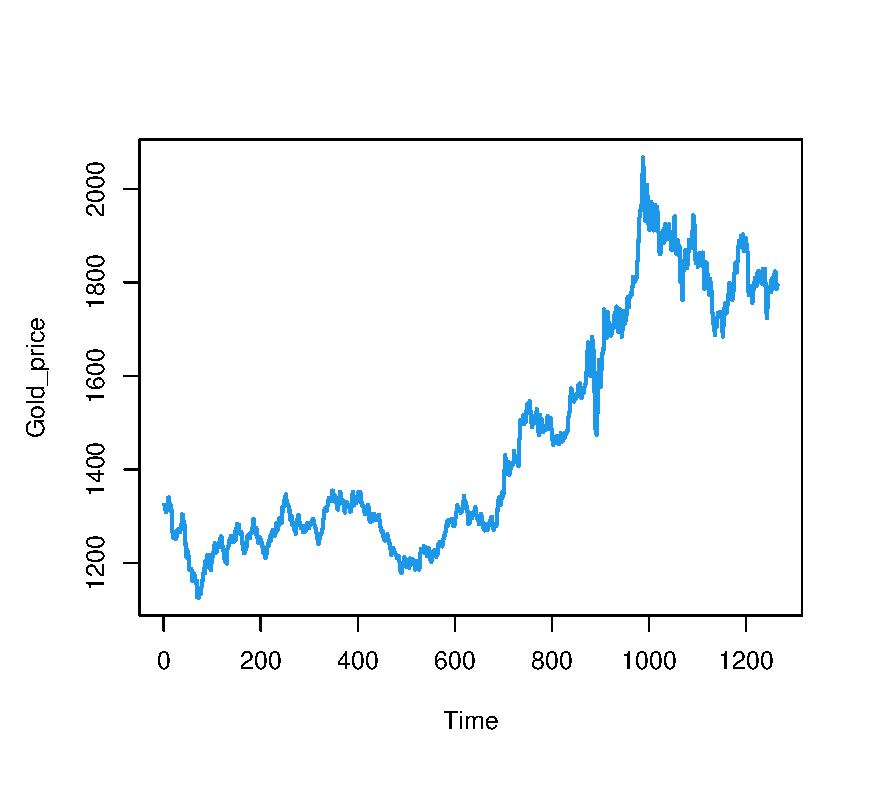
\includegraphics[height=2.75in]{D:/meisai/ms/fig/fig3G.eps}
  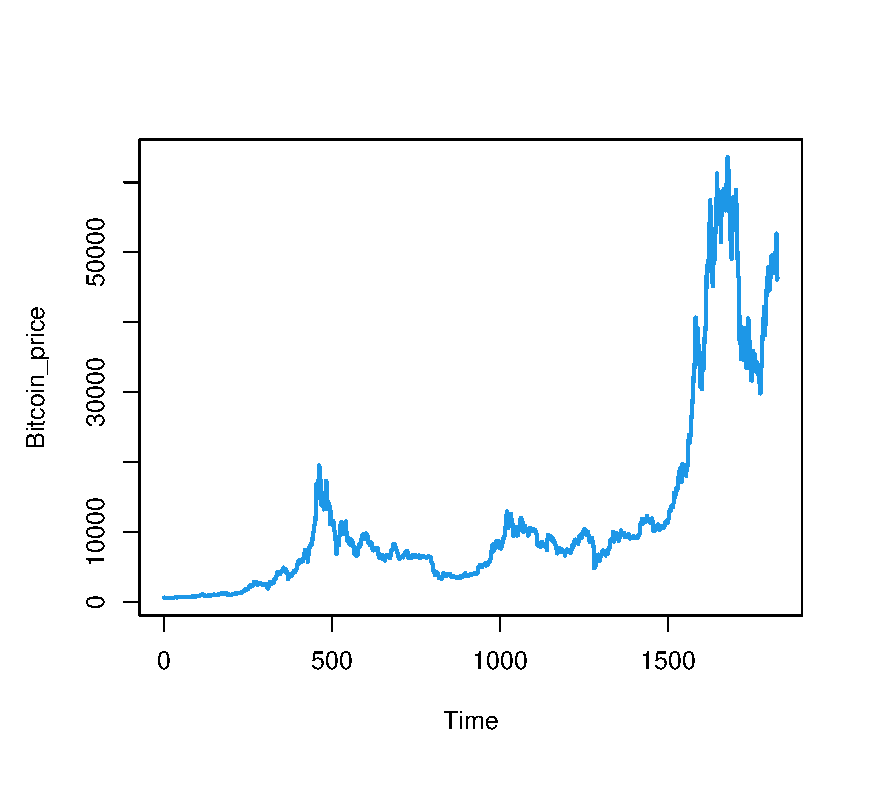
\includegraphics[height=2.75in]{D:/meisai/ms/fig/fig3b.eps}
  \caption{Raw data visualization} \label{fig3}
\end{figure}


Testing unit root,and result is shown below:

%一阶差分
Secondly,the first-order difference data is obtained according to the first-order difference of the original data, 
and the two methods abrove are also used to test.The result is as follows.\ref{fig4}
\begin{figure}[!hb]
  \centering 
  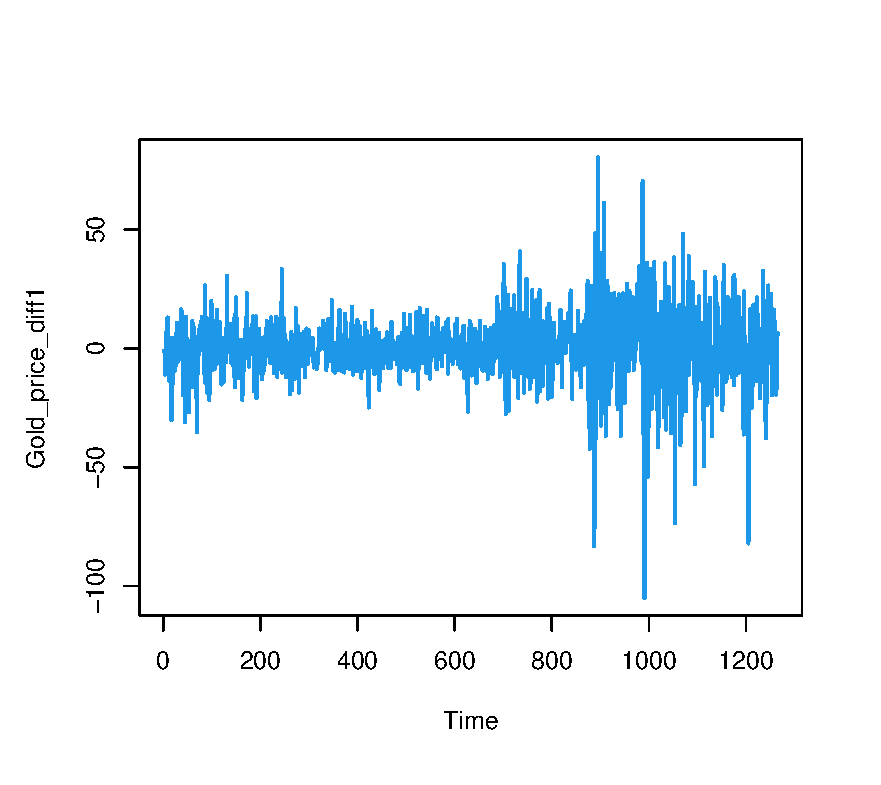
\includegraphics[height=2.75in]{D:/meisai/ms/fig/gd1.eps}
  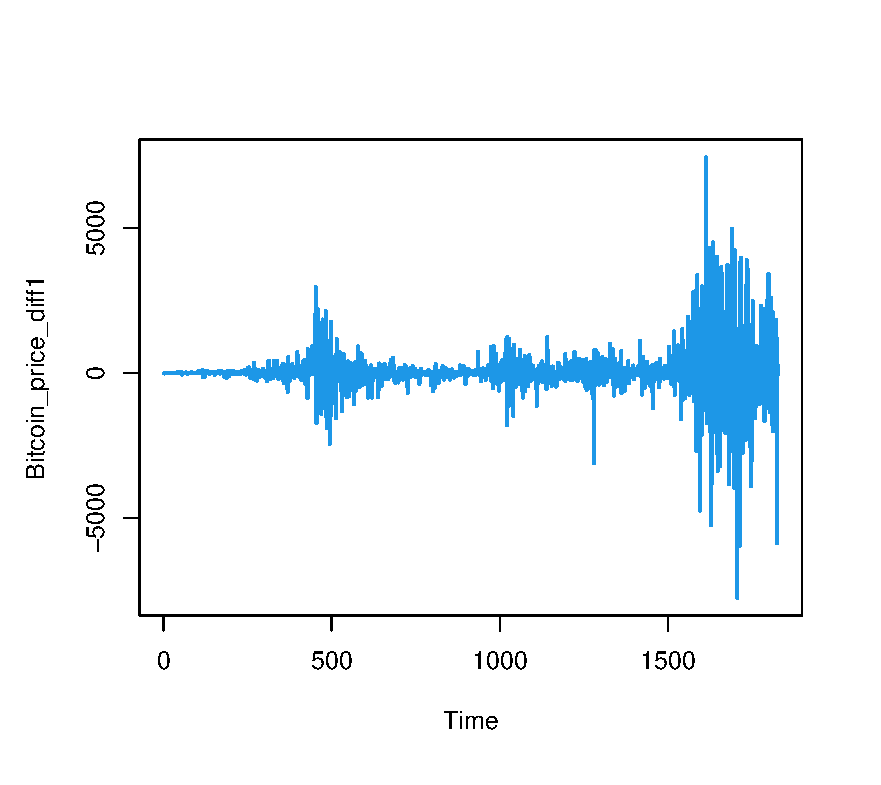
\includegraphics[height=2.75in]{D:/meisai/ms/fig/bd1.eps}
  \caption{first order difference data} \label{fig4}
\end{figure}



%二阶
Thirdly,utilizing second order difference we obtained second order difference data with two methods testing
The result is shown in\ref{fig5}.
\begin{figure}[!h]
  \centering 
  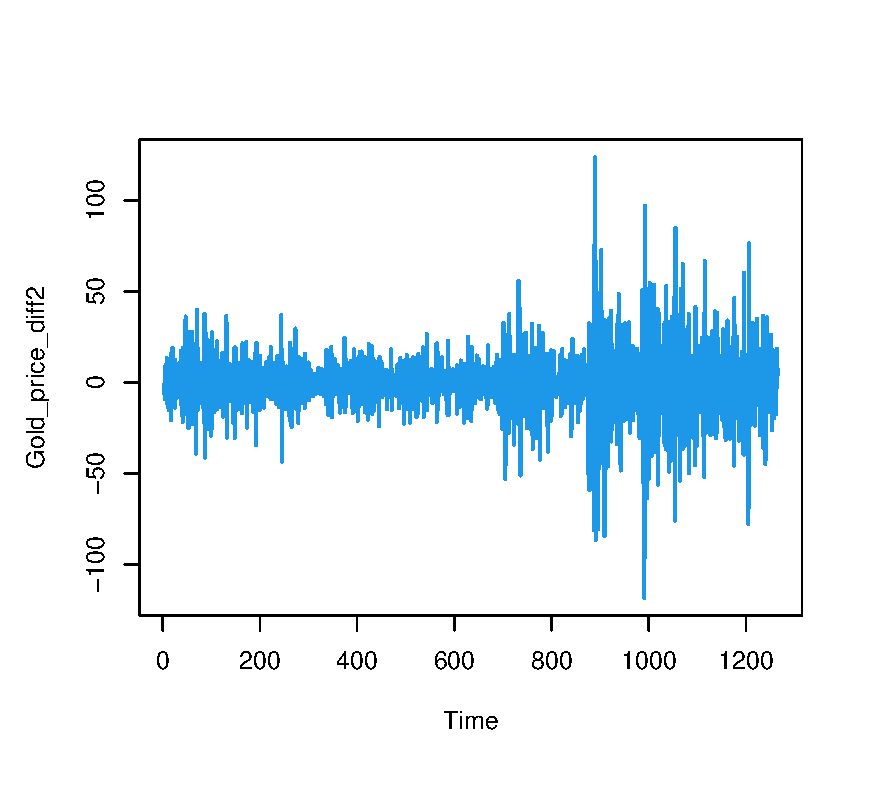
\includegraphics[height=2.75in]{D:/meisai/ms/fig/gd2.eps}
  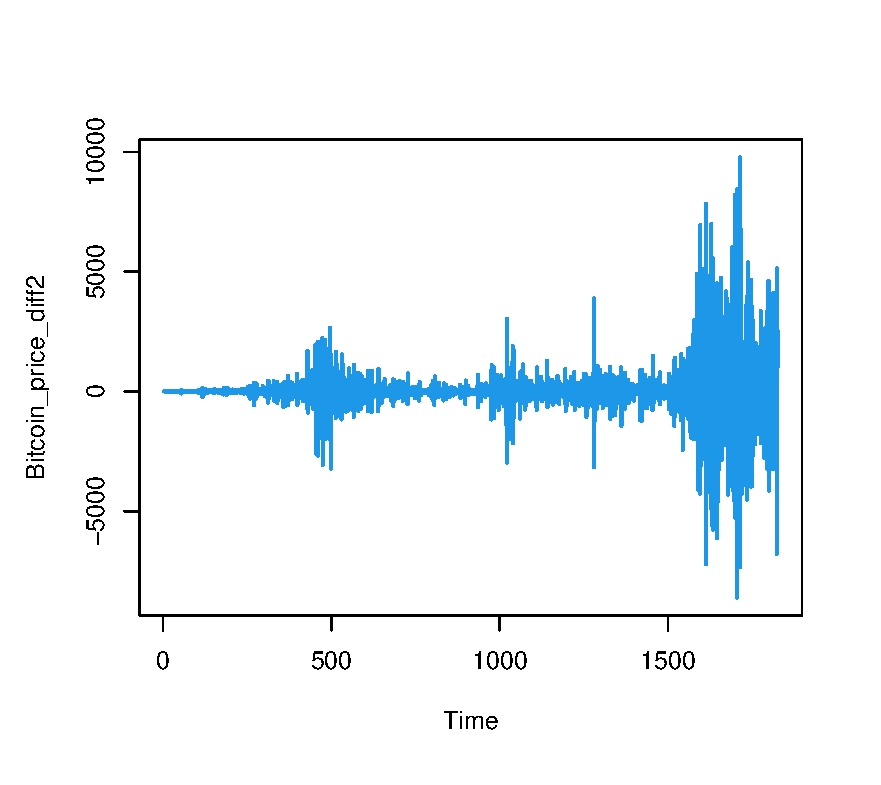
\includegraphics[height=2.75in]{D:/meisai/ms/fig/bd2.eps}
  \caption{second order difference data} \label{fig5}
\end{figure}


%白噪音检验
\subsubsection{White Noise Test}
We need to evaluate whether the data is white noise or not, 
and will discard the one that is white noise because it has no research significance.
So We chose Ljung-Box test to meet the demands.

The first step is to examine the raw data,The test yielded the following graph

The second step,we test first order difference data,result can be seen below

Third,we test second order difference data,result is shown below


%第一问
\section{PartⅠ:Model Development }
\subsection{Time Series Model ARIMA - Data Forecasting }
\subsubsection{Model Theory}
Autoregressive Integrated Moving Average model is the differential integrated moving average autoregressive model, 
also known as the integrated moving(or slilding)average autoregressive model, 
is one of the time series forecasting analysis methods. 
In ARIMA(p, d, q),AR is "autoregressive", p is the number of autoregressive terms;
MA is "sliding average ",q is the number of sliding average terms, and d is the number of differences (order) made to make it a smooth series.
Although the word "difference" does not appear in the English name of ARIMA, it is a key step to analyse time series.
%补充公式
%确定系数pq
\subsubsection{Determining the parameters p, q }
We take advantage of the autocorrelation and partial autocorrelation plots to find out the parameters p, q.
The following figures show the the format of autocorrelation and partial autocorrelation plots.
\begin{figure}[!h]
  \centering 
  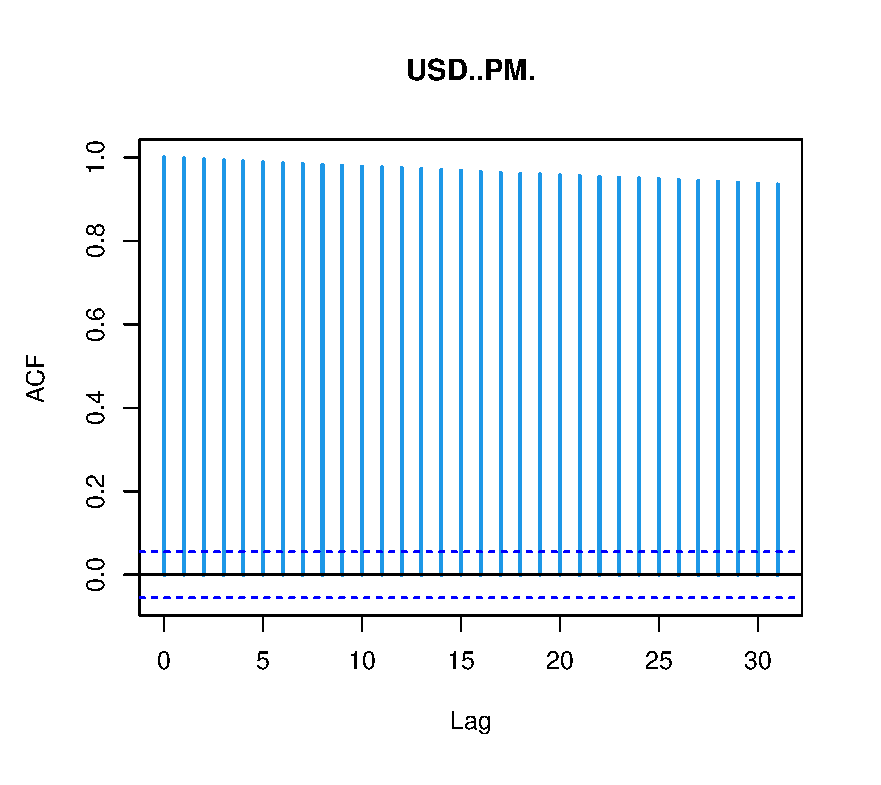
\includegraphics[height=2.75in]{D:/meisai/ms/fig/g6.eps}
  \caption{Autocorrelation diagram}
  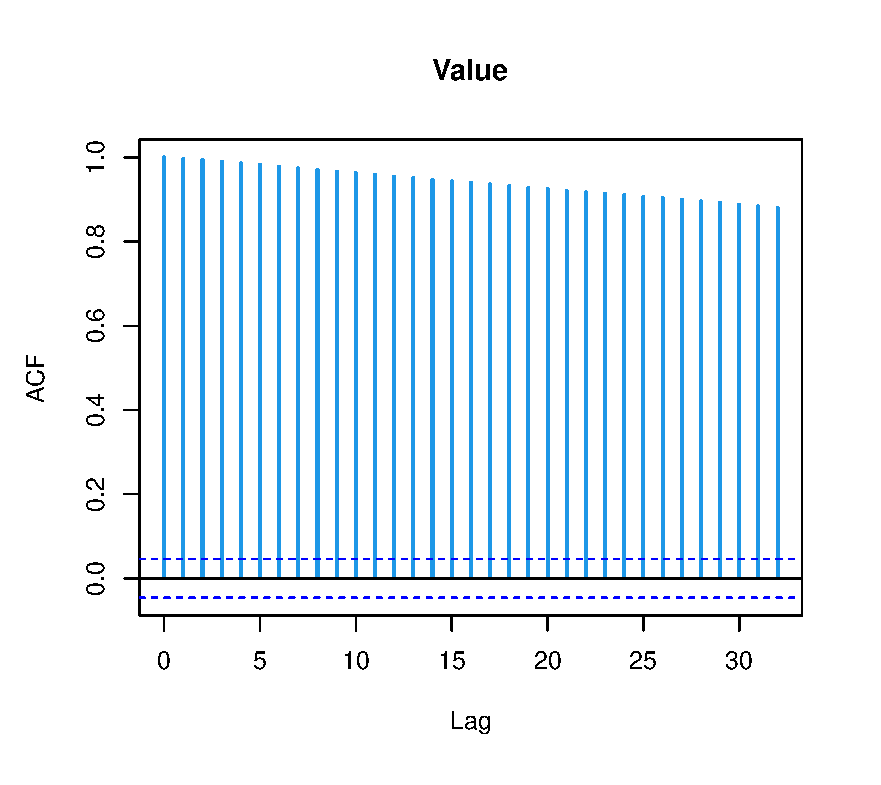
\includegraphics[height=2.75in]{D:/meisai/ms/fig/b6.eps}
  \caption{Partial autocorrelation diagram} \label{fig6}
\end{figure}

In theory
Tail-dragging: always have non-zero values, not constant equal to zero after k is greater than some constant (or fluctuate randomly around 0).

Truncated tail: After greater than a constant k, it quickly tends to 0 as a k-order truncated tail when both autocorrelation and partial.

By figure \ref{fig4}and \ref{fig5}, it can be seen that the first order difference data and the second order difference data are meaningful time series.
Therefore,we use the same methods in the subsequent section.The analysis charts are as follows.

\begin{figure}[htbp]
  \centering
  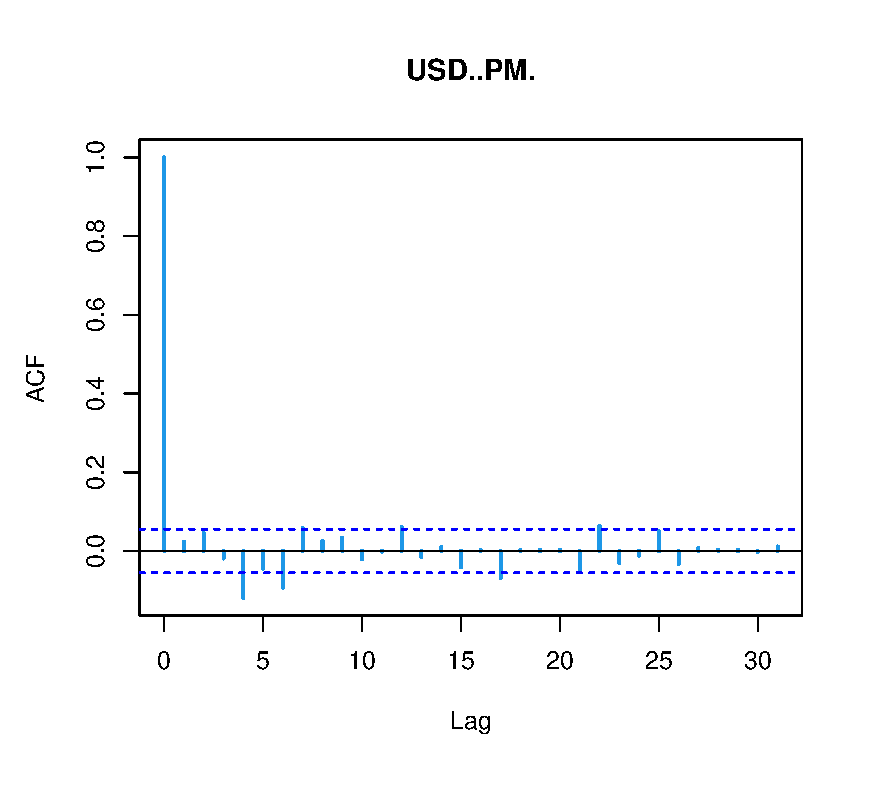
\includegraphics[height=2.5in]{D:/meisai/ms/fig/g61.eps}
  \caption{First order differential autocorrelation diagram-gold}
  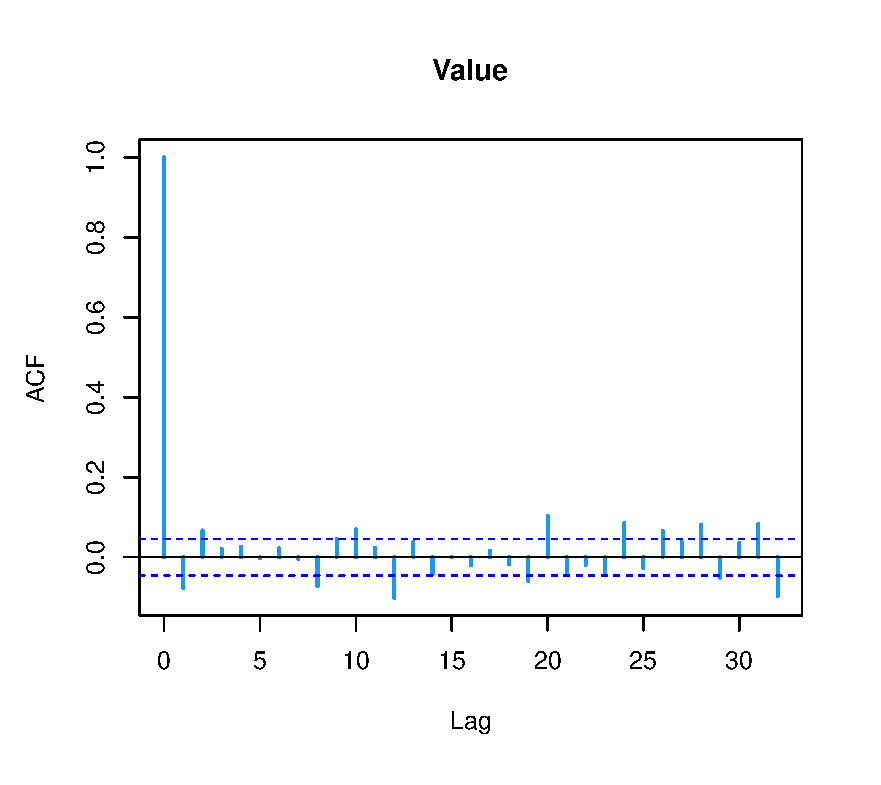
\includegraphics[height=2.5in]{D:/meisai/ms/fig/b61.eps}
\end{figure}
\begin{figure}[htbp]
  \caption{First order differential partial autocorrelation diagram-bitcoin} 
  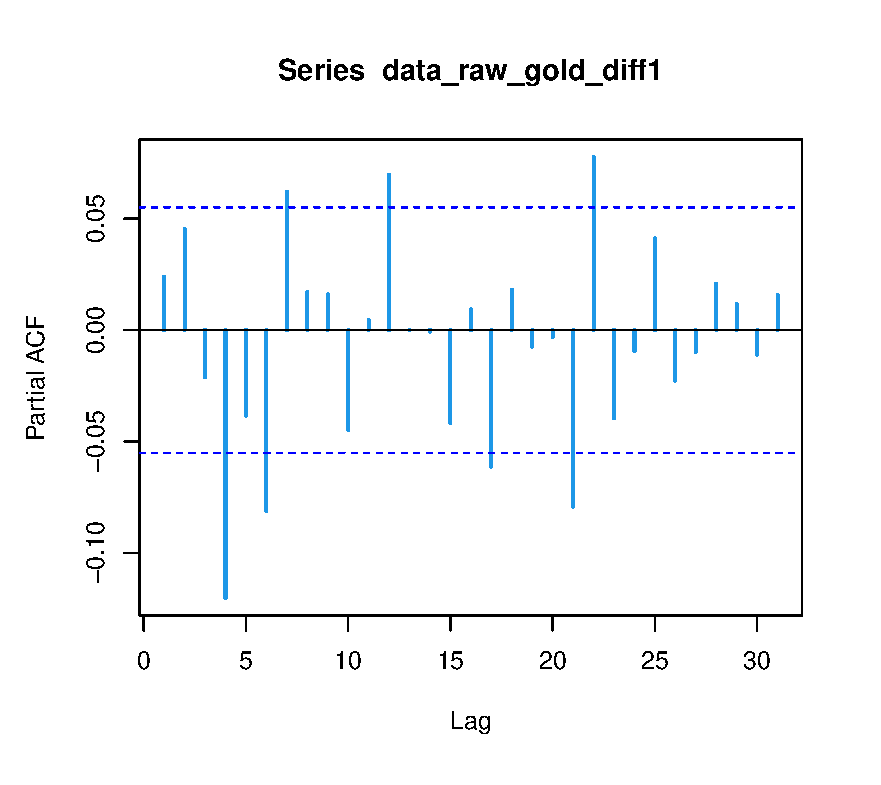
\includegraphics[width=3cm]{D:/meisai/ms/fig/g661.eps}
  \caption{First order differential autocorrelation diagram-gold}
  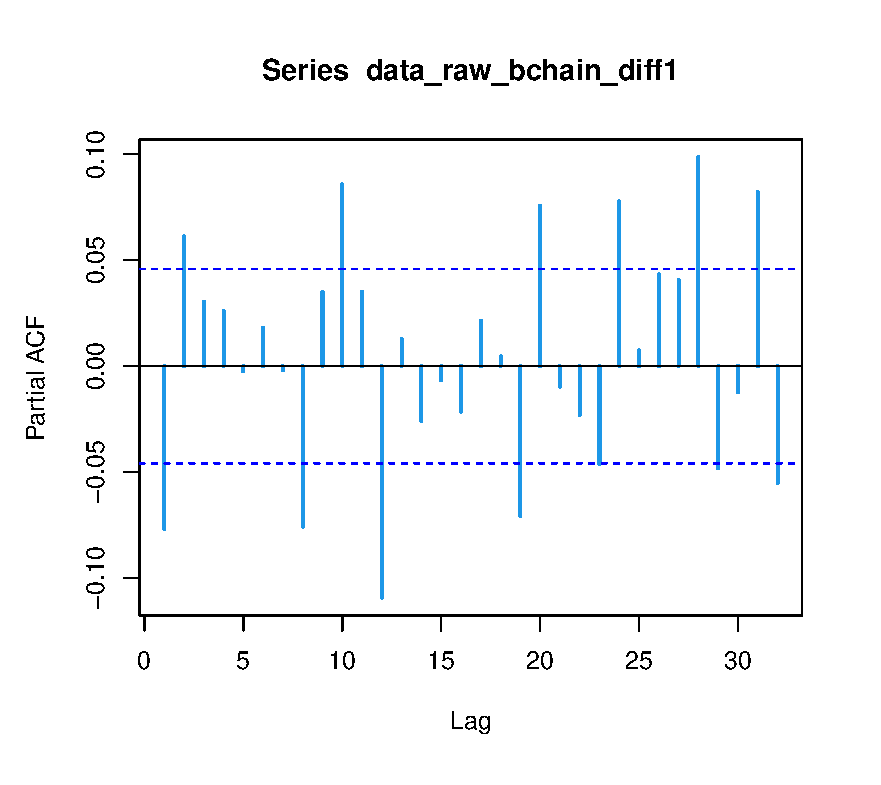
\includegraphics[width=3cm]{D:/meisai/ms/fig/b661.eps}
  \caption{First order differential partial autocorrelation diagram-bitcoin} 
\end{figure}

\begin{figure}[!h]
  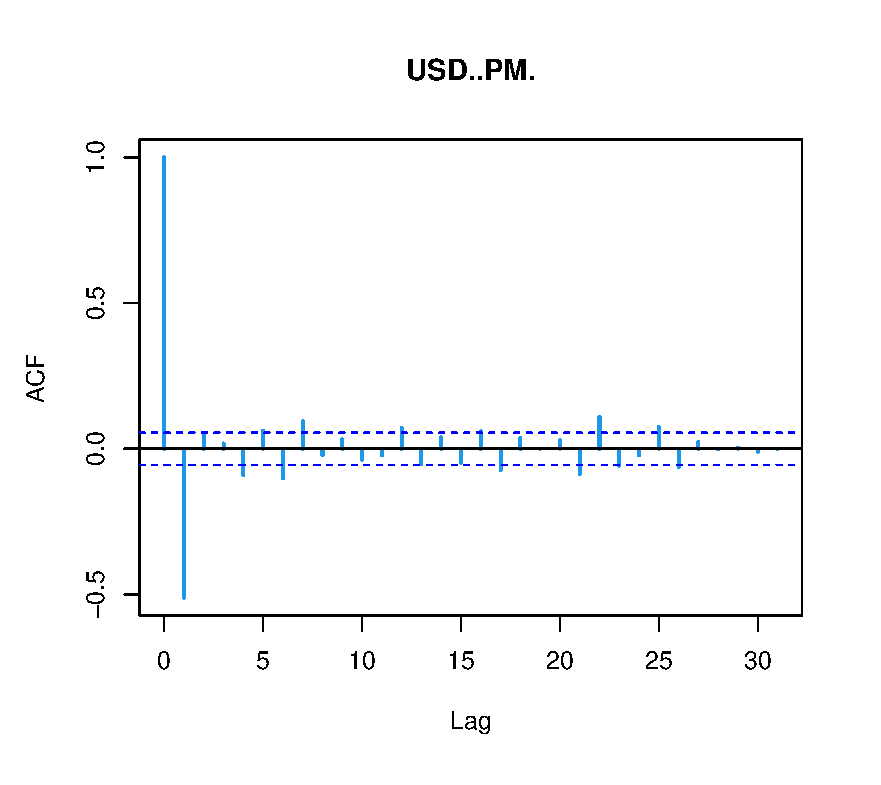
\includegraphics[height=2.4in]{D:/meisai/ms/fig/g62.eps}
  \caption{Second order differential autocorrelation diagram-gold}
  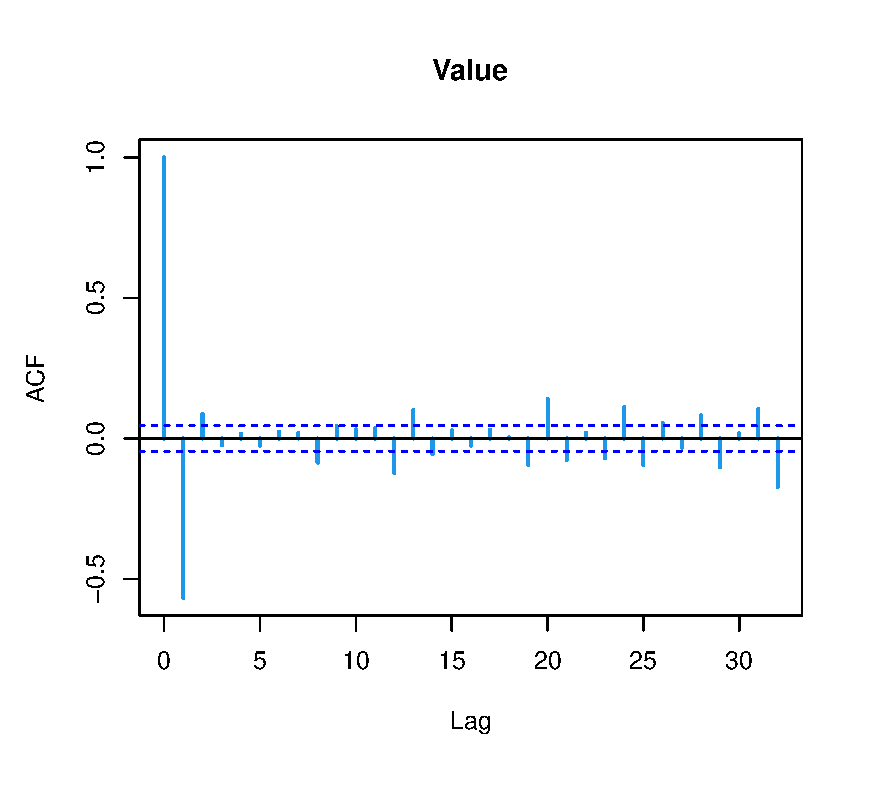
\includegraphics[height=2.4in]{D:/meisai/ms/fig/b62.eps}
  \caption{Second order differential partial autocorrelation diagram-bitcoin} 
  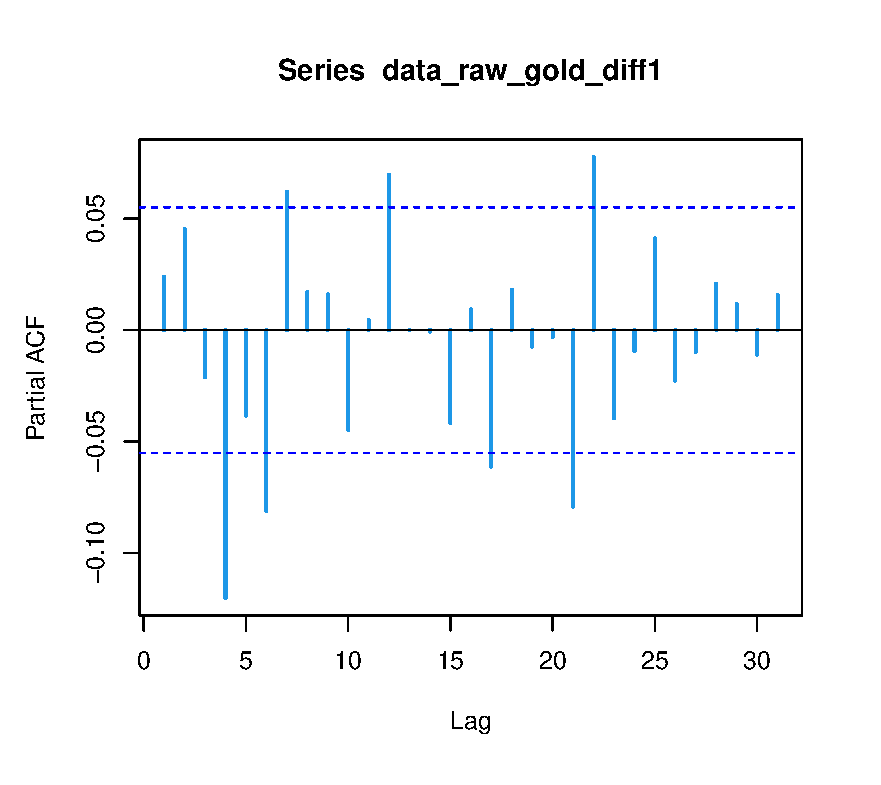
\includegraphics[height=2.4in]{D:/meisai/ms/fig/g661.eps}
  \caption{Second order differential autocorrelation diagram-gold}
  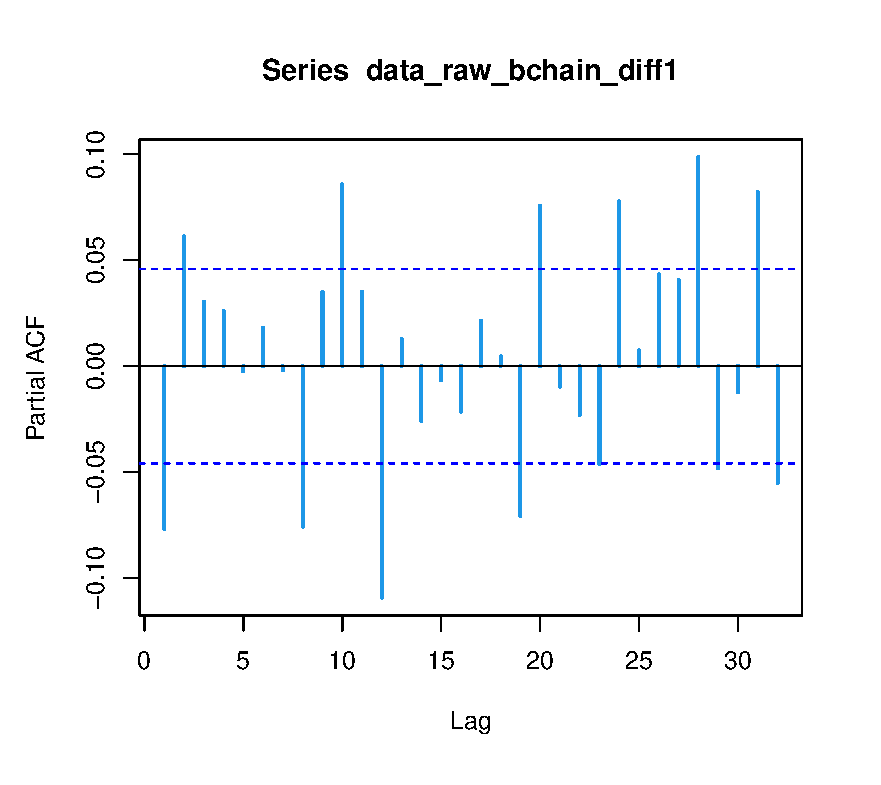
\includegraphics[height=2.4in]{D:/meisai/ms/fig/b661.eps}
  \caption{Second order differential partial autocorrelation diagram-bitcoin} 
  \label{fig661}
\end{figure}


%R语言确定
\subsubsection{R Language Determines the Optimal Parameters p, d, q}
Given that only the price data as of the day can be used each day, i.e., 
the training data used each day are inconsistent,
it is not practical to determine the optimal parameters for the model through autocorrelation and partial autocorrelation plots, 
so we use the auto.arima function in R language to automate the parameter determination.

The best model information was obtained after using the auto.arima function with all given data.
And the model is as follows:



%模型残差白噪声检验
\subsubsection{White noise test for model residuals}
It is usually assumed that the model residuals of a reasonable model should be white noise.
logically we conducted a white noise test on the residuals of the resulting model.
The results are as follows.



\subsubsection{Model Prediction and Visualization}
To make the results more intuitive,we use the model to calculate and predict the historical data. 
And the visualization results are shown in the figure
<<<<<<< HEAD


The reason for the large overlap of lines in Figure 6 is that the data sample is too large.
So we choose 100 of these samples and make graph7.

\subsubsection{Batch prediction of data}   %去未来七天
Based on the price data as of the day,we predicted gold and bitcoin price for the next 7 days 
and the same automated arima modeling is performed using the auto.arima function to obtain the price data for the next 7 days.
By analyzing the forecast data, we observed a roughly linear variation. 
Then,we integrated these data using linear regression to clarity the future price trend 
and fitted slope quantifies the trend to make the better investment decisions.

=======
>>>>>>> 2c96c476387fffaab53ed17cec63ad83775b1903


The reason for the large overlap of lines in Figure 6 is that the data sample is too large.
So we choose 100 of these samples and make graph7.

\subsubsection{Batch prediction of data}   %去未来七天
Based on the price data as of the day,we predicted gold and bitcoin price for the next 7 days 
and the same automated arima modeling is performed using the auto.arima function to obtain the price data for the next 7 days.
By analyzing the forecast data, we observed a roughly linear variation. 
Then,we integrated these data using linear regression to clarity the future price trend 
and fitted slope quantifies the trend to make the better investment decisions.



\subsection{Trading Strategy Model - Dynamic Programming }
符号说明:
$w_G$:持有黄金的比例
$w_B$:持有比特币的比例
$r_G$:黄金预期收益率
$r_B$:比特币预期收益率
$\alpha _G$:交易黄金时的佣金比例
$\alpha _B$:交易比特币时的佣金比例
$\sigma _G$:黄金的历史收益率的下半方差
$\sigma _B$:比特币的历史收益率的下半方差
$\beta $:交易者的风险厌恶系数
$T$:每次购买资产后持有的平均天数

%流程图


\subsubsection{资产的预期收益情况}
当购买和卖出资产时需要支付一定比例的佣金,换句话说,每天持有资产是有成本的,可以用$\alpha \div T$表示。
当预期收益大到足以抵消这个成本时,就可以考虑买入。当预期收益小于负的成本时,代表持有
该资产的亏损额即将超过成本,需要立刻抛出止损。

如果$r>(1+\beta )\alpha \div T$,代表该资产近期会涨,可以买入。

如果$r<-(1-\beta )\alpha \div T$,代表该资产近期会跌,必须卖出。

如果$-(1-\beta )\alpha \div T<r<(1+\beta )\alpha \div T$,代表资产近期价格稳定,不需要买也不需要卖。


moreover,由于投资者、投资产品的不同,投资方对于风险有不同的厌恶程度,因此我们引入了$\beta $来刻画风险厌恶程度。
$\beta $越大,表示投资者越保守,买入的限制更严格,卖出的限制更宽松。反之,表示投资者越激进,他有更宽松的买入标准
和更严格的卖出标准。

此外,在购买时我们不得不考虑下面两种情况:
\begin{enumerate}
  \item 如果黄金和比特币中只有一种达到了上涨条件,那么我们只需要把当前的可用资金全部买入该资产即可。
  \item 而如果黄金和比特币同时上涨,就需要考虑如何分配可用资金。在这种情况下,我们采用夏普比率衡量不同比例投资组
  合的好坏程度。
  $$ Sharpe \; Ratio=\frac{w_G\times r_G+w_B\times r_B}{\sqrt{w_G^2 \sigma _G^2 + w_B^2 \sigma _B^2+2Cov_{w_B w_G}}}$$
  我们用下半标准差作为衡量风险的量化指标,作为标准差中代表小于均值的波动的部分,它更能体现资产亏损的风险。
  用预期收益率除下半标准差得到夏普比率,它意味着当前投资组合每一单位风险所对应的收益大小。当夏普比率最大时,无疑
  意味着当前比例的投资组合是最优的。

  根据“每次购买时消耗所有现金”和“黄金和比特币的价格波动相互独立”这两个假设,我
们可以利用计算机求出投资组合最优时的两种资产比例的数值解。这是如下的优化问题:
\begin{align*}
  max \qquad & \frac{w_G\times r_G+w_B\times r_B}{\sqrt{w_G^2 \sigma _G^2 + w_B^2 \sigma _B^2}\\
  s.t. \quad & w_G+w_B=1\\
  & 0 \le w_G \le 1 \\
\end{align*}
\end{enumerate}


\subsubsection{当前的资产持有情况}

\subsubsection{Positioning Standard Identification}

\subsubsection{Daily Portfolio Determinations}






\section{PartⅡ:Strategy Evaluation}
\subsection{Set Perturbation Terms }%to determine optimal parameters }

\subsection{Comparison Illustrates the Best Strategy}




\section{PartⅢ:Sensitivity Analysis}
\subsection{Assuming Changes In Commission}

\subsection{Visualization Results}%Analysis ensitivity}





\section{Evaluate of the Model}
\subsection{Strengths and weaknesses}

\subsection{Sensitivity Analysis}




\section{Conclusions}


\section{A Memo}








\begin{thebibliography}{99}
\bibitem{1} D.~E. KNUTH   The \TeX{}book  the American
Mathematical Society and Addison-Wesley
Publishing Company , 1984-1986.
\bibitem{2}Lamport, Leslie,  \LaTeX{}: `` A Document Preparation System '',
Addison-Wesley Publishing Company, 1986.
\bibitem{3}\url{https://www.latexstudio.net/}
\end{thebibliography}

\begin{appendices}

\section{First appendix}

In addition, your report must include a letter to the Chief Financial Officer (CFO) of the Goodgrant Foundation, Mr. Alpha Chiang, that describes the optimal investment strategy, your modeling approach and major results, and a brief discussion of your proposed concept of a return-on-investment (ROI). This letter should be no more than two pages in length.







\begin{letter}{Dear, Mr. Alpha Chiang}

\vspace{\parskip}

Sincerely yours,

Your friends

\end{letter}
Here are simulation programmes we used in our model as follow.\\

\textbf{\textcolor[rgb]{0.98,0.00,0.00}{Input matlab source:}}
\lstinputlisting[language=Matlab]{./code/mcmthesis-matlab1.m}

\section{Second appendix}

some more text \textcolor[rgb]{0.98,0.00,0.00}{\textbf{Input C++ source:}}
\lstinputlisting[language=C++]{./code/mcmthesis-sudoku.cpp}

\end{appendices}
\end{document}
%% 
%% This work consists of these files mcmthesis.dtx,
%%                                   figures/ and
%%                                   code/,
%% and the derived files             mcmthesis.cls,
%%                                   mcmthesis-demo.tex,
%%                                   README,
%%                                   LICENSE,
%%                                   mcmthesis.pdf and
%%                                   mcmthesis-demo.pdf.
%%
%% End of file `mcmthesis-demo.tex'.